\documentclass{article}

\usepackage{amsmath}
\usepackage{amssymb}
\usepackage{graphicx}
\usepackage{xcolor}
\usepackage{hyperref}
\usepackage{booktabs}
\usepackage{tabularx}

\hypersetup{colorlinks=true,
			linkcolor=blue,
			filecolor=magenta,
			urlcolor=cyan,
}

\urlstyle{same}

\title{SE 3XA3: Development Plan\\Staroids}

\author{Team 20, Staroids
		\\ Moziah San Vicente, 400091284, sanvicem
		\\ Eoin Lynagh, 400067675, lynaghe
		\\ Jason Nagy, 400055130, nagyj2
}

\date{Friday September 28, 2018}

%\input{../Comments}

\begin{document}

\begin{table}[hp]
\caption{Revision History} \label{TblRevisionHistory}
\begin{tabularx}{\textwidth}{llX}
\toprule
\textbf{Date} & \textbf{Developer(s)} & \textbf{Change}\\
\midrule
Sept 21 & Eoin, Jason, Moziah & Added questions to be answered\\
Sept 23 & Jason & Added communication plan and team member roles\\
Sept 23 & Eoin & Added coding style\\
Sept 23 & Jason & Added git workflow\\
Sept 23 & Moziah & Added technology and temporary Excel Gantt Chart\\
Sept 24 & Eoin and Jason and Moziah & Divided PoC work and polished\\
Sept 25 & Jason & Added planned modules and menus\\
Sept 27 & Moziah & Added third party tools\\
Sept 28 & Eoin & Added team meeting plan and feasibility\\
Sept 28 & Jason & Tidied up document and fixed problematic merge\\
Sept 28 & Moziah & Architecture updated Gantt chart\\
\textcolor{red}{Nov 28 & Jason & Spelling corrections}\\
%Note: You cannot write '&' in the above table because that marks a new column. You must also end the line with '\\'
\bottomrule
\end{tabularx}
\end{table}

\newpage

\maketitle

This document was created to gather all the information required to manage the development of the Staroids software project. It is to be used as an aid throughout the project and encloses a number of development decisions that have been decided during the inception phase of the project, and will be maintained throughout it.

\section{Team Meeting Plan}
%Eoin
Meetings will be held in CNH basement, at 17:30, as well as using the time spent in labs to further the goals of the project.\\
The scribe will be Eoin Lynagh, he will be responsible for the completion of meeting minutes at each meeting.\\
The chair will be Jason Nagy, he will be responsible for making sure all necessary work is divvied up as well as making sure that meetings remain on task.\\
The meeting minutes will record the meeting date, location and time, as well as information regarding meeting goals, work that has been done since the last meeting, reporting on what has been slowing down progress. It will also contain notes on the meeting, and what work has to be done, as well as who has to do it.\\

\section{Team Communication Plan}
%Jason
Most work related jobs and tasks will be discussed through Facebook Messenger. The aforementioned discussion includes assigning work, talking about current issues, discussing what is next and how implementations should be done. Facebook Messenger will be used in addition to the scheduled meetings. The meetings will be about larger issues while Facebook Messenger will have simpler issues. If someone is unable to use Facebook Messenger for whatever reason, email can also be used for casual work discussion. Some examples of issues that are Facebook Messenger worthy are bugs in the program, code portions where the coder is unsure how to solve a problem, letting the team know what someone is currently working on.\\
For more time critical issues, the phone is to be used. It can be through text or call, but call is preferred because it allows for synchronous communication. Some example issues worth of phone communication include questions for work that are due soon and application crashing bugs, should they occur.\\
The members of Staroids have all exchanged phone and Facebook information.\\

\section{Team Member Roles}
%Jason
The leader of Staroids will be Jason. As leader, he is responsible for organizing meetings and giving deadlines.\\
The scribe of Staroids will be Eoin. Eoin is in charge of meeting agendas and ensuring meeting documents are current and accurate. He is also responsible for assembling the meeting agendas from information from everyone.\\
The technology expert and submitter will be Moziah. Moziah is responsible for researching and implementing new technologies and tools to be used in the project while also ensuring that the Git repo is maintained properly. Moziah will also ensure the final versions of files are properly tagged.\\
As a group, Staroid members will collectively discuss and decide what the next tasks to complete are and who shall be assigned which parts, depending on why has what relevant skills.

\section{Git Workflow Plan}
%Jason
Staroids has decided to use branching for this project. All Staroid members will have their own personal branches that will be periodically merged with the master. If any one member needs help from another, they can simply switch to their branch and then switch back once the issue has been resolved. Major versions will be based on milestones and minor versions will not be used. All major milestones will also be tagged from within Git. Milestones will both be project deliverables as well as group decided features. Another technology that is planned to be used is the Atom text editor's "Tele-type" functionality. This allows multiple members to simultaneously work on the same file from different computers. The main use of this tool will be for helping each other with problematic pieces of code.\\

\section{Proof of Concept Demonstration Plan}

%Sources:\\ https://en.intechcore.com/proof-of-concept-in-software-development/\\ https://sensinum.com/proof-of-concept-in-software-development/\\

%Jason
Staroids is planned to have four modules that contain the content of the game. The first module, and most basic, is the "Utilities" module. This fundamental module will contain functions that are needed by more than two other modules. This ensures that all other modules that share commands draw from one source, instead of using their own version. This will reduce the required code in each of the modules. The second module is the "Game Object" module which will contain all of the intractable objects within the game. This includes the player ship, asteroids and the enemy alien. This module will make use of the Utilities module. The structure of the module will include a base "Game Object" class which contains fundamental attributes that all game objects share, like an x and y coordinate, a sprite among others. The specialized objects will then inherit the base class and will then be specialized to fulfill their role. The third module will be a brief sound module, aptly named "Sound". It will contain the source and initializations for any sound files that are used. Lastly, the fourth module will be the "Game State" module, which will contain the object that runs all other module and represents the actual game. It will contain all game logic required for the other modules to interact with each other.\\
There are also four main states planned for Staroids that will enable the user to play the game comfortably. First, there will be an opening screen. This menu will have a prompt for the user to press a button to start the game. In this menu, the game is not active and there is no way to lose the game. Its purpose is so that the player can get ready to play and is not immediately thrusted into the game on program launch. The second menu is the pause screen. This menu will simply suspend the game state and allow for resuming at the click of a button. The button to resume the game will be shown in an on-screen prompt and the words "Paused" will appear somewhere on the screen. The final game state is "Game Over". This screen occurs only when the user has run out of lives and loses the game. The words "Game Over" will show in the centre of the screen and a button to restart will be shown. Lastly, while not strictly a menu, the "Playing" state will have constant information for the user. The majority of the screen will be taken up by the game, but in the top right corner of the screen, there will be a life count and score. These amounts can always be seen, no matter what menu the user is in and will always appear above game objects that happen to pass over the text.\\

%Moe
The only third party tools that will be used in the demonstration are the internet browsers to test the program on, specifically Apple Safari, Microsoft Edge, Firefox, and Google Chrome. This is to show that the implementation is compatible with all major web browsers. All other third part tools that are being used throughout the project development are described in the \hyperref[technology:ide]{technology section} of the document.\\

%Eoin
The Staroids team has studied the technical feasibility of our product, and believe that the project is feasible. First, many programs and tools are available to help project development. Atom has built in packages to test JavaScript, and testing can be done through internet browser software. The Staroids team also have experience working with JavaScript, so language wise, this project is not beyond our programming abilities. Testing graphics and sounds, although new to two of the group members, will also be possible due to the diverse experience within the team.\\
The Staroids team also believes that our project is buildable within the time frame given. Using a combination of Atom and Git, prototyping will be done quickly and effectively while keeping the code intact. Working with Git will help with keeping changes separate and with assuring that no major deletions or loss of work can occur.\\
Throughout the project separation of concerns, modularity, abstraction, anticipation of change and incremental development will be followed to ensure that the best product is produced.

\section{Technology}
%JavaScript - Canvas
%HTML5
%Case based?
%LaTeX (pdflatex)
\subsection{Programming Language}
The programming language that was chosen to use for this project is JavaScript. As JavaScript is a web developing language, the project will be able to run on websites, which is a large benefit because it will allow the Staroids application to reach many more people than if it had to be downloaded. Also JavaScript makes it easier to run since no setup is required for the user, all that is needed is to go to a website that hosts the game or open the HTML file that contains Staroids. Next, the original program that Staroids is based upon is also written in JavaScript so there is a guide to reference when developing Staroids. Completing this project will also expose Staroids members to a language that has not been used in the Software Engineering program at McMaster University.
\subsection{IDE}
\label{technology:ide}
The IDE that will be used for Staroids is Atom. Atom is one of the most widely used IDE’s for coding in a broad array of languages. While not made specifically for JavaScript, it is still rated a top five JavaScript IDE according to \href{https://jaxenter.com/top-5-javascript-ide-146609.html}{Jaxenter}. Other good features about Atom that will be useful for the development of Staroids is it’s Git integration, as well as the ability to work on the same files together on different computers using its portal feature.
\subsection{Testing Framework}
The testing framework that will be used is a combination of two frameworks called Mocha (Testing Framework) and Chai (Assertion Library). This is one of the most widely used JavaScript testing frameworks, and has a built in integration with Atom to make testing as convenient and straightforward as possible.
\subsection{Document generation}
All documentation will be written in \LaTeX, as specified in the course outline, and will then have a pdf generated from the \LaTeX file. The only exception to this will be for the documentation of the code, where JsDoc will be used to autogenerate the pdf documentation based on comments. This is because it is a popular and widely used documentation tool for JavaScript and has many tutorials and lots of information online, such as \href{https://milmazz.uno/article/2014/08/27/how-to-document-your-javascript-code/}{milmazz}.

\section{Coding Style}
%Eoin
\subsection{File Names}
File names will be written using camel case, and will use a descriptive title. For example, the title of this document is styleGuidelines.
\subsection{Variable Names}
Variable names will be written using camel case, and will be written as follows baseAttributeDescriptor, so for example, a variable representing the velocity of a ball would be named velocityBall.
\subsection{Javascript}
Javascript code will be written to follow the \href{https://google.github.io/styleguide/jsguide.html}{Google JavaScript Style Guide}, which details coding standards for source code in JavaScript. However, the style of Variable/File names is described above, and may not follow the Google Style guide.

\section{Project Schedule}
%Moe
%Provide a pointer to your Gantt Chart.
The Gantt chart can be found in the Project Schedule folder under the file name: "StaroidsGantt.gan".
%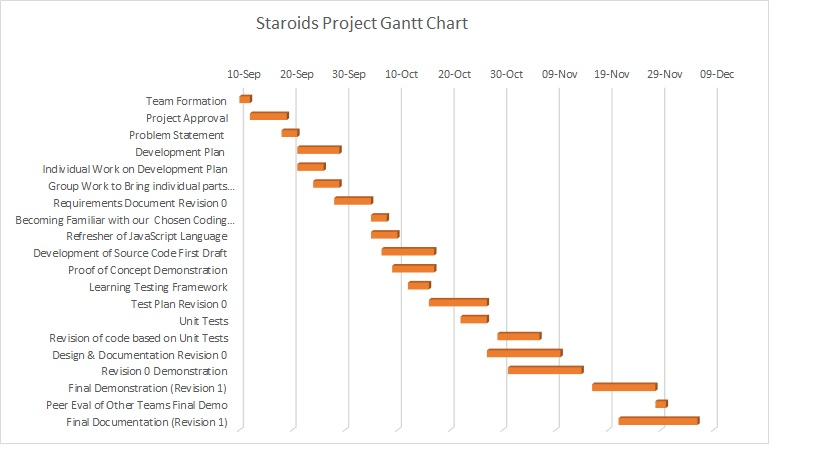
\includegraphics[scale=0.75]{gantt.jpg}

\section{Project Review}
%Leave blank for now

\bibliographystyle{plainnat}

\bibliography{DevelopmentPlan}

\end{document}
